\documentclass[base.tex]{subfiles}
\begin{document}
\paragraph{Exemple d'application}
Ensemble $\mathbb{Q}$ des nombres rationnels est dénombrable.
\[\mathbb{Q}=\{\frac{a}{b}| a \in \mathbb{Z} , b \in \mathbb{Z}_+ , pgcd(a,b)=1\}\]
\[\mathbb{Q}=\{(a,b)| a \in \mathbb{Z} , b \in \mathbb{Z}_+ , pgcd(a,b) = 1 \} \subseteq \mathbb{Z}^2 \leftrightarrow \mathbb{N}\]
$\mathbb{N}$ est aussi en bijection avec un sous ensemble de $\mathbb{Q}$ qui est $\mathbb{N}$ lui même : $\mathbb{N} \subseteq \mathbb{Q}$

      \begin{figure}[!h]
         \centering
         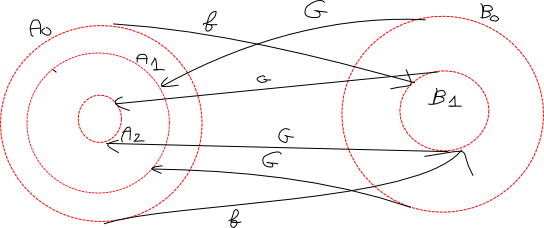
\includegraphics[scale=0.8]{path3556}
      \end{figure}

Il y a une bijection entre $\mathbb{A}_2 \subseteq \mathbb{A}_1 \subseteq \mathbb{A}_0$ et il y a une bijection entre $\mathbb{A}_0 $ et $\mathbb{A}_2$ . Elle s'obtient en appliquant d'abord $f$ puis $g$. \\
\\
Un énoncé équivalent au théoreme de Cantor-Bernstein :\\
Si $\mathbb{A}_2 \subseteq \mathbb{A}_1 \subseteq \mathbb{A}_0$ , et s'il existe une bijection entre $\mathbb{A}_0$ et $\mathbb{A}_2$ ,alors il existe une bijection entre $\mathbb{A_0}$ et $\mathbb{A}_1$ ($\mathbb{B_0}$ peut être désormais oublié).\\
\\
En répétant les fonctions $f,g,f,g,...$ . On obtient les choses suivantes :
\[\mathbb{A}_0 \supseteq \mathbb{A}_1 \supseteq \mathbb{A}_2 \supseteq \mathbb{A}_3 \supseteq ... \supseteq \mathbb{D} \]
$\mathbb{D}$ peut être vide ou non . Et il existe des bijections :
\[\mathbb{A}_0 \rightarrow\mathbb{A}_2 \rightarrow\mathbb{A}_4 \rightarrow \mathbb{A}_6\rightarrow ...\]
\[\mathbb{A}_1 \rightarrow\mathbb{A}_3 \rightarrow\mathbb{A}_5 \rightarrow \mathbb{A}_7\rightarrow ...\]
%schéma 2 feuille 1
\[C_0=\mathbb{A}_0\setminus\mathbb{A}_1\]
\[C_1=\mathbb{A}_1\setminus\mathbb{A}_2\]
Les "couches" $C_i,i=0,1,2,...$ sont disjoints.\\
Il y a des bijections :
\[C_0 \rightarrow C_2 \rightarrow C_4 \rightarrow C_6 \rightarrow ...\]
\[C_1 \rightarrow C_3 \rightarrow C_5 \rightarrow C_7 \rightarrow ...\]
et pas d'union puisqu'il n'y a pas de parties communes.
\\
\\
\[\mathbb{A}_0 = C_0 + C_1 + C_2 + C_3 + D\]
\[\mathbb{A}_1 =       C_1 + C_2 + C_3 + D\]
Pour les pairs $\searrow$ bijection\\
Pour les impair $\downarrow$ bijection (identité)
\subsubsection{Une deuxième application de la diagonalisation}
Soit $\mathbb{P}$ l'ensemble des programmes qui prennent en entrée un entier $x \in \mathbb{N}$ et qui retournent en sortie un $y\in \mathbb{N}$.\\
Tout programme comme cela peut être codé comme une suite fini de bits. Donc $\mathbb{P}\subseteq \{0,1\}^*$, et par conséquent $\mathbb{P}$ est dénombrable (voir ex 1.12 ) . \\
Les éléments de $\mathbb{P}$ peuvenet être numéroté
\[\mathbb{P} = \{p_0,p_1,p_2,p_3,p_4,p_5,...\}\]
et tout les programme de $\mathbb{P}$ figurent dans cette liste infinie.\\
Le résultat d'application de $p$ à $x$ sera noté
\[y=p(x)\]
Une subtilité , un programme une fois lancé peut ne jamais s'arrêter et donc ne pas donner de résultat.\\
\\
$p(x)$ est aussi une fonction $\mathbb{N} \rightarrow \mathbb{N}$ mais cette fonction est \underline{partielle}, c'est à dire qu'elle peut être non définie pour certains $x$. \\
\\
On dit qu'une fonction est partiellement calculable s'il existe un programme qui la calcule .\\
Une fonction nulle part définie est calculable !\\
\\
Une fonction est totale si elle est définie pour tout $x \in \mathbb{N}$ . Etre partielle est une permission et non pas une obligation.\\
\\
Construisons la table suivante
%schéma 3 feuille 1
\\
\\
A cause du fait que certains programmes peuvent ne jamais aboutir , il y a des "trous" (les cases vides) dans la table .\\
Alors faisons par exemple :\\
Soit $\bar{p}(x)=p(x) $ si $p$ ayant été appliquer à $x$ s'arrête .\\
$\bar{p}(x) = 0$ sinon \\
\\
\textbf{Remarque}\\
Les fonctions totales ne changent pas .\\
\\
Soit $h(n)$ la fonction suivante :
\[h(n)=\bar{p}_n(n)+1\]
Nous avons supposé qu'il y ait tous les programmes qu'il soit dans la colone $p_0,p_1,2,...$ et par conséquent toutes les fonctions calculables dans les lignes de la table , et on est arrivé à une contradiction . La fonction h ne figure pas dans la table !!!

\paragraph{Le problème de l'arrêt}
Instance : $(p,x):p\in \mathbb{P} , x\in \mathbb{N}$\\
Question : Le programme $p$ ; ayant été appliqué à $x$ s'arrête t'il ?\\
Le problème de l'arrêt est indécidable !\\
\\
Il n'existe pas d'algorithme qui puisse dire , pour tout programme $p\in\mathbb{P}$ et pour toute donnée $x\in\mathbb{N}$ si $p$ appliqué à $x$ s'arrête ou non.
\end{document}
